\documentclass{article}
\usepackage{graphicx} % Required for inserting images
\usepackage{amsmath}
\usepackage{amssymb}
\usepackage{amsthm}
\usepackage{tikz}
\title{BA476}
\author{Yunzhe Yu}
\date{February 2024}

\begin{document}

\maketitle

\section*{Problem 1}
\begin{itemize}
    \item [(a)]
        % Accuracy calculation
        The logistic regression model is given by:
        \[
        \log\left(\frac{p}{1-p}\right) = \beta_0 + \beta_1 X1 + \beta_2 X2
        \]
        where \( \beta_0 = 0.6 \), \( \beta_1 = 3 \), and \( \beta_2 = -0.1 \).
        
        Solving for \( p \) (the probability) gives us:
        \[
        p = \frac{e^{\beta_0 + \beta_1 X1 + \beta_2 X2}}{1 + e^{\beta_0 + \beta_1 X1 + \beta_2 X2}}
        \]
        
        Using a threshold \( t = 0.5 \), we find the accuracy of the model to be 80\%.

    \item[(b)] 
        % Alternative threshold calculation
        To find an alternative threshold to maximize accuracy, we look for a threshold between the incorrectly predicted probability (approximately 0.52) and the closest higher correct probability (approximately 0.79). An alternative threshold at the midpoint of these values is approximately 0.655.

    \item[(c)]
        % Odds calculation
        For a predicted probability of \( p(x) = 0.7 \), the odds of observing label 1 are given by \( \frac{p(x)}{1 - p(x)} \), which is approximately 2.33.

    \item[(d)]
        % Interpretation of the coefficient
        For the final part, since \( e^{\beta_1} = e^3 \) increases the odds, the statement that having \( X1 = 1 \) increases your odds of having label 1 by \( \beta_1 = 3 \) is "True."
\end{itemize}
\newpage

\begin{itemize}
    \item [(a)]
\begin{tikzpicture}[level 1/.style={sibling distance=20em},
                    level 2/.style={sibling distance=15em},
                    level 3/.style={sibling distance=8em},
                    every node/.style = {shape=rectangle, draw, align=center}]

  \node {\(X_1 \leq 0.4\)}
    child { node {\(X_2 < 0.2\)}
      child { node {R2} }
      child { node {R1} }
    }
    child { node {\(X_1 < 0.6\)}
      child { node {R4} }
      child { node {\(X_2 < 0.6\)}
        child { node {R5} }
        child { node {R3} }
      }
    };
\end{tikzpicture}

    \begin{figure}
        \centering
        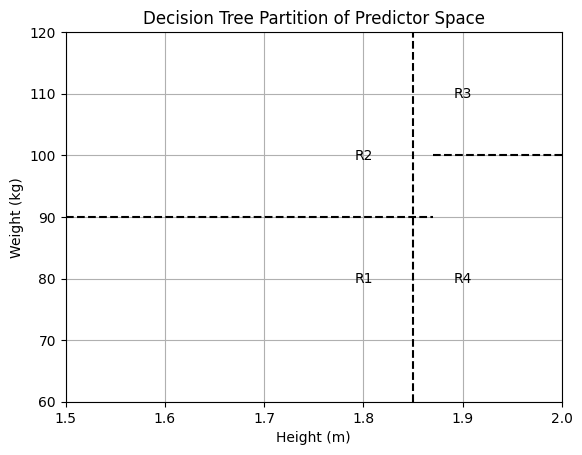
\includegraphics[width=1\linewidth]{hw3-p2.png}
        \label{fig:enter-label}
    \end{figure}
\end{itemize}
\newpage

\section*{Problem 3}

\begin{itemize}
    \item Tree (a) has 3 misclassification.
    \item Tree (b) has 4 misclassifications.
    \item Tree (c) has 2 misclassifications.
\end{itemize}

\begin{enumerate}
    \item[(a)] The initial split of Tree (c) makes the fewest mistakes as it has the lowest number of misclassifications (2).
    \item[(b)] Number of instances incorrectly classified in each of the three trees:
    \begin{itemize}
        \item Tree (a) misclassifies 3 instances.
        \item Tree (b) misclassifies 4 instances.
        \item Tree (c) misclassifies 2 instances.
    \end{itemize}
    \item[(c)] The number of splits \( |T| \) in each tree:
    \begin{itemize}
        \item Tree (a) has 2 splits.
        \item Tree (b) has 1 split.
        \item Tree (c) has 0 splits.
    \end{itemize}
    \item[(d)] The tree selected by cost-complexity pruning when \( \alpha = 0.5 \) is Tree (c).
    \item[(e)] The tree selected by cost-complexity pruning when \( \alpha = 2 \) is also Tree (c).
\end{enumerate}

\section*{Problem 4}
\begin{itemize}
    \item For the first datasets(leftmost), X3 could be X1 * X2 such that X3 $<$ 0 would give the instance red(1) and X3 $>$ 0 give the instance black(0).
    
    \item For the second datasets(middle), X3 could be $|X1|$ which is the absolute value of X1. 
    
    \item For the third datasets(rightmost), X3 could be $|X1|$ + $|X3|$ since it’s in linear pattern and involved in both positive and negative coefficients.
\end{itemize}

\section*{Problem 5}
\begin{enumerate}
    \item 
    The first tree \( f_1 \) is trained on a bootstrap sample selected by the sequence (5, 1, 6, 5, 2, 3) and utilizes 'Age' and 'Tightness\_in\_chest' as predictors. The decision tree finds the optimal split at an 'Age' of 56 years. The rules are as follows:
\begin{itemize}
    \item If Age \( \leq 56 \): predict \texttt{False} for Cardiac Arrest.
    \item If Age \( > 56 \): predict \texttt{True} for Cardiac Arrest.
\end{itemize}

    \item 
The second tree \( f_2 \) is trained on a bootstrap sample selected by the sequence (3, 2, 1, 2, 6, 5) and uses 'ECG' and 'Tightness\_in\_chest' as predictors. The decision tree finds the optimal split using the 'ECG' predictor. The rules are:
\begin{itemize}
    \item If ECG \( \leq 0.5 \): predict \texttt{False} for Cardiac Arrest (corresponds to 'Normal').
    \item If ECG \( > 0.5 \): predict \texttt{True} for Cardiac Arrest (corresponds to 'Hypertrophy' or 'Abnormal').
\end{itemize}

    \item 
    The third tree \( f_3 \) is trained on a bootstrap sample selected by the sequence (2, 2, 4, 1, 1, 5) and uses 'Bp\_change' and 'Tightness\_in\_chest' as predictors. Despite the presence of a split on 'Bp\_change', the tree concludes that all instances predict a cardiac arrest. The rule is:
\begin{itemize}
    \item Predict \texttt{True} for Cardiac Arrest for any value of 'Bp\_change'.
\end{itemize}

    \item 
    \begin{enumerate}
    \item \textbf{Instance 1} (Age = 79, ECG = Hypertrophy):
    \begin{itemize}
        \item $f_1$: True (Age $>$ 56)
        \item $f_2$: True (Hypertrophy)
        \item $f_3$: True
        \item \textbf{Aggregated}: True (Majority is True)
    \end{itemize}

    \item \textbf{Instance 2} (Age = 51, ECG = Normal):
    \begin{itemize}
        \item $f_1$: False (Age $\leq$ 56)
        \item $f_2$: False (Normal)
        \item $f_3$: True
        \item \textbf{Aggregated}: False (Majority is False)
    \end{itemize}

    \item \textbf{Instance 3} (Age = 48, ECG = Abnormal):
    \begin{itemize}
        \item $f_1$: False (Age $\leq$ 56)
        \item $f_2$: True (Abnormal)
        \item $f_3$: True
        \item \textbf{Aggregated}: True (Majority is True)
    \end{itemize}

    \item \textbf{Instance 4} (Repeated Instance 1):
    \begin{itemize}
        \item \textbf{Aggregated}: True
    \end{itemize}

    \item \textbf{Instance 5} (Age = 79, ECG = Hypertrophy):
    \begin{itemize}
        \item \textbf{Aggregated}: True
    \end{itemize}

    \item \textbf{Instance 6} (Age = 77, ECG = Normal):
    \begin{itemize}
        \item $f_1$: True (Age $>$ 56)
        \item $f_2$: False (Normal)
        \item $f_3$: True
        \item \textbf{Aggregated}: True (Majority is True)
    \end{itemize}
\end{enumerate}
\break


\end{enumerate}



    \begin{figure}
        \centering
        \includegraphics[width=1\linewidth]{utput.png}
        \label{fig:enter-label}
    \end{figure}
    
\textbf{(b)}
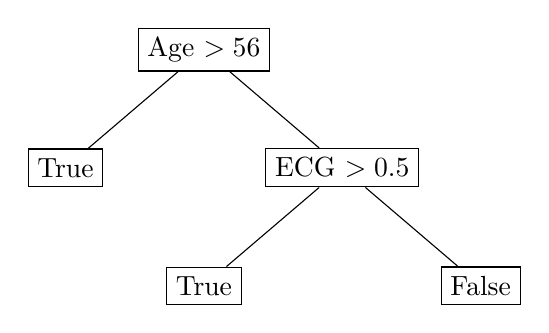
\begin{tikzpicture}[sibling distance=10em,
  every node/.style = {shape=rectangle, draw, align=center}]
  \node {Age \( > 56 \)}
    child { node {True} }
    child { node {ECG \( > 0.5 \)}
      child { node {True} }
      child { node {False} } };
\end{tikzpicture}
\newpage

\section*{Problem 7}
\begin{enumerate}
    \item[(a)] The current algorithm does not satisfy demographic parity, equality of opportunity, or individual fairness with the threshold \( t = 0.5 \). The positive prediction rate for Group A is \(83.33\%\) and for Group B is \(50\%\), which are not equal, thus failing to meet demographic parity. The true positive rate for Group A is \(100\%\) and for Group B is \(50\%\), not satisfying equality of opportunity. And, the prediction rate for outcomes 0 and 1 are \(60\%\) and \(80\%\), respectively, indicating a potential issue with individual fairness.

    \item[(b)] Finding a threshold that satisfies demographic parity or equality of opportunity without trivial decisions requires a careful balancing act, which might not be possible with a single threshold applied uniformly to all groups.

    \item[(c)] Potential biases in the training process could include imbalanced training data, features correlating with group membership, or past biases reflected in the outcome variable.
\end{enumerate}




\end{document}